\section{Sparsity in DNN Training}
 \label{sec:sparse_dnn_training}
 
 We motivate our work and project the benefits of our optimizations for DNN training.  First, we provide intutition into why sparsity exists in DNN training.  Next, using a real-world image recogntion workload, we empirically demonstrate the amount of sparsity that exists in practice.  Finally, we discuss how available sparsity can be exploited using our techniques to improve training efficiency. 
 
\subsection{Sources of Sparsity}
\label{subsec:sparsity_source}

Machine learning experts have long observed that DNN training using back-propagation and gradient descent involves a considerable amount of computation on sparse data structures~\cite{Ng04, Nair10, Krizhevsky12, Bengio13, Srivastava14a} (i.e., data structures that contain a significant fraction of zeroes).  Specifically, performance-critical data of training, such as error gradients and weight deltas, can exhibit noticeable levels of sparsity during training.   Some of the sparsity arise naturally from the training algorithm  and the underlying matrix multiplication kernels.  For example, correct predictions of a neuron's output activation during feed-forward evaluation results in zero-valued neuron error gradients, during back-propagation, which can introduce sparsity in the rest of the network.  Beyond this, standard techniques for boosting training quality often introduce additional sparsity in the network.  These include techniques such as Rectified Linear Units (ReLUs)~\cite{Nair10, Krizhevsky12} for faster convergence, and  L$_1$~\cite{Ng04, Bengio13} and Dropout~\cite{Srivastava14a} regularization methods for reducing overfitting. 

\subsection{Sparsity in Real-word Image Recognition}
\label{subsec:sparsity_profile}

To provide insight into the amount of sparsity that exists in real-world DNN training workloads, we profile the training of a DNN model on the standard {\it CIFAR-10} image recognition task~\cite{KrizhevskyThesis} (described in ~\ref{subsec:eval_method}).  In our study, we reason about sparsity from two perspectives: (i) computation sparsity and (ii)  data sparsity.  Computation sparsity measures the percentage of mutiply-add operations that are performed on zero values in the performance-critical phases of training (e.g., feed-forward evaluation), while data sparsity measures the percentage of zeroes in the input data (e.g., activations) of these phases.  Both perspectives are useful because they capture different impacts of sparsity on system performance, and motivate different optimization opportunities.  Computation sparsity captures the impact on processing cycles, data sparsity captures the impact on memory capacity, and both metrics capture the impact on memory bandwidth.  We measure both sparsity metrics over $10$ training epochs using the standard training data set of $60000$ images. 

\begin{figure*}
 \centering
 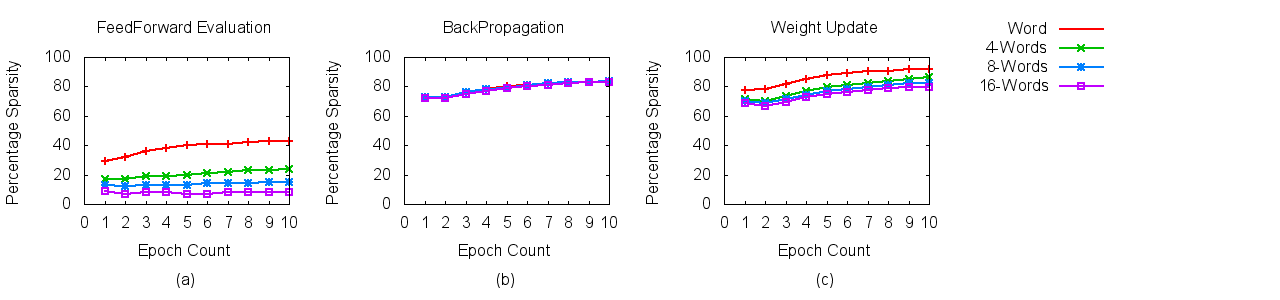
\includegraphics[width=1.9\columnwidth]{Figures/multi_computesparsity.png}
\caption{Computation sparsity in CIFAR-10 image recognition training.}
 \label{fig:cifar-10_compute_sparsity}
 \end{figure*}
 
\subsubsection{Computation Sparsity}
\label{subsec:computation_sparsity}
 Figure~\ref{fig:cifar-10_compute_sparsity} reports computation sparsity in the key phases of DNN training for the first $10$ epochs of training a CIFAR-10 image recognition model.  Since computation sparsity represents opportunities to safely reduce processing cycles, Figure~\ref{fig:cifar-10_compute_sparsity} reports sparsity for different computation granularities to show the potential benefits for non-vectorized (i.e., {\it Word}) and vectorized (e.g., {\it 4-Words}) implementations of the computation kernels.  For example, for feed-forward evaluation, {\it Word} sparsity is the percentage of CPU multiply-adds that can be skipped because one of the input activation or weight values is zero, while {\it N-Words} sparsity is the percentage of N-wide vector (SIMD) multiply-adds that can be skipped because either the $N$ activation values or $N$ weight values are zero. 
 
We make the following four observations regarding computation sparsity in DNN training from Figure~\ref{fig:cifar-10_compute_sparsity}.  First, considerable sparsity exists in all the training phases: {\it Word} sparsity is $29\%$---$43\%$ for feed-forward evalution, $73\%$---$84\%$ for backpropagation, and $77\%$--$92\%$ for weight updates.   Second, the training phases have different amounts of computation sparsity, with feed-forward evaluation having the least amount of computation sparsity. Third, computation sparsity generally \emph{increases} with epoch count.  Fourth, vectorization affects computation sparsity of the training phases in different ways: vectorization has no impact on sparsity for backpropagation, but reduces sparsity modestly for weight updates and significantly for feed-forward evaluation (e.g., {\it 4-Words} sparsity is half of {\it Word} sparsity).  In summary, the results shows there is potential to greatly reduce the processing and memory bandwidth requirements of DNN training by exploiting computation sparsity, but vectorization limits the benefits for feed-forward evaluation. 

%Fourth, the impact of vectorization on computation sparsity varies across the training phases: no impact for backpropagation, modest sparsity reduction for weight updates, and significant sparsity reduction for feed-forward evalution (e.g., {\it 4-Words} sparsity is half of {\it Word}).  In summary, the results shows there is potential to greatly reduce the processing and memory bandwidth requirements of DNN training by exploiting computation sparsity, but vectorization limits the benefits for feed-forward evaluation. 
  
 \begin{figure*}
 \centering
 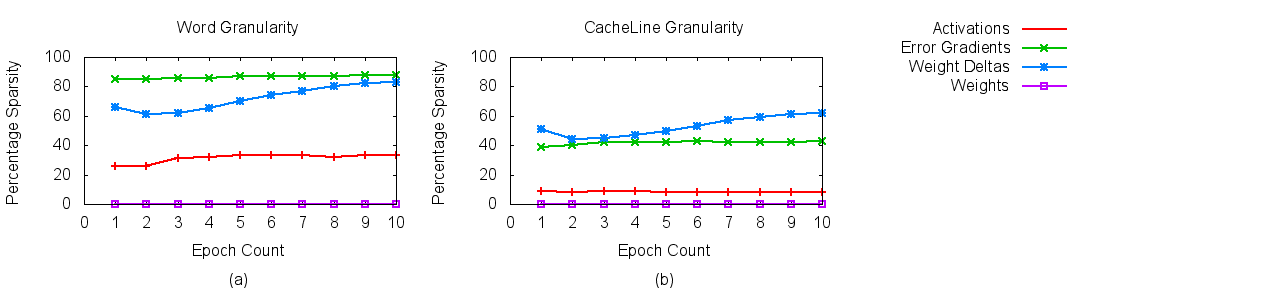
\includegraphics[width=1.9\columnwidth]{Figures/multi_datasparsity.png}
\caption{Data sparsity in CIFAR-10 image recognition training.}
 \label{fig:cifar-10_data_sparsity}
 \end{figure*}

\subsubsection{Data Sparsity} 
\label{subsec:data_sparsity}
Figure~\ref{fig:cifar-10_data_sparsity} reports the sparsity of the different performance-critical data in DNN training: (i) activations, (ii) error gradients, (iii) weight deltas, and (iv) weights (defined in Section~\ref{subsec:dnn_training}).  The results are presented for word and cacheline granularities.  Data sparsity at word granularity is the percentage of individual data values (e.g., activations) which are zeroes, while cacheline granularity is the percentage of data cache lines containing only zeroes.  Since training data values are represented with 4-byte floats, the $64$-byte cacheline granularity represents clusterings of $16$ sparse data values.  Viewing data sparsity at both word and cacheline granularities helps one understand the trade-offs of different optimization strategies since significantly more expensive hardware is required to track sparsity at word granularity compared to cacheline granularity.  

We make the following three observations regarding data sparsity in DNN training from Figure~\ref{fig:cifar-10_data_sparsity}.  First, sparsity level varies across the different data items: at word granularity, weights have $0\%$ sparsity (i.e., dense), while activations ($26\%$---$33\%$), error gradients ($83\%$---$85\%$), and weight deltas ($66\%$---$83\%$) are considerably sparse.   Second, for the sparse data items, sparsity tends to increase with more training epochs.  Third, sparsity levels are reduced at cacheline granularity to about half of word granularity, which suggests poor clustering of sparse data values in the data layout of the workload.  However, considerable levels of sparsity \emph{stil}l remain at the cacheline granularity.  In summary, the results show that cache capacity and bandwidth requirements of DNN training can be greatly reduced by exploiting data  sparsity, even at the relatively large cacheline granularity.

\subsection{Optimization Opportunities}
\label{subsec:sparse_code_oppor}
We motivate our hardware optimizations for sparse computations and data in DNN training by studying a performance-critical kernel for computing weight deltas in back-propagation.  Figure~\ref{fig:deltas_source_code} illustrates a simplified version of this kernel.\footnote{Our approach also applies to vectorized (e.g., SIMD) kernels, but we use the simple forms in our discussion for convenience.}   The weight deltas of a layer in the DNN are computed by the inner product of the neuron activations and error gradients.  Given the amounts of computation and data sparsity in training, a promising optimization for this kernel is to skip the multiply-add operations if either \emph{activations[i]} or \emph{errors[j]} is zero.  Moreover,  if \emph{errors[j]} is zero, the inner loop can be skipped entirely since \emph{errors[j]} is loop-invariant. These optimization ideas also apply to the other performance-critical kernels of training, e.g., feed-forward evalution. 

\begin{figure}[h]
 \centering
 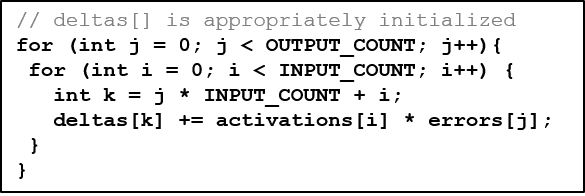
\includegraphics[width=.9\columnwidth]{Figures/deltas_source_code.png}
\caption{Code snippet for computing weight deltas.}
 \label{fig:deltas_source_code}
 \end{figure}

Although these optimizations could be implemented in software by checking the data values for zero and guarding computations based on those checks, such a software approach has a couple of practical limitations.   First, it requires software changes which might not be possible for existing binaries.   Second, the required software checks incur both computation and memory overheads, which could be significant and outweigh the optimization benefits.  For example, checking \emph{activations[i]} and checking \emph{errors[j]} for zeroes have different performance impact.  Checking \emph{errors[j]} for zeroes is likely to be beneficial because it can be done \emph{outside} the inner loop, and helps to skip large amounts of computation. In contrast, checking \emph{activations[i]} for zeroes will likely hurt performance because it occurs \emph{inside} the inner loop, and can save only a small amount of computation. 

\subsection{Overview of our Hardware Optimizations}
\label{subsec:overview}
In this work, we propose hardware optimizations for improving DNN training performance by exploiting sparsity in performance-critical computations and data of training workloads. Our harware mechanisms are designed to avoid the limitations and overheads of a software approach.   Our approach consists of low cost extensions to the processor and memory systems.  Our processor extensions exploit computation sparsity to \emph{safely} skip instructions that compute on sparse data thereby reducing the compute requirements of  DNN training (Section~\ref{sec:processor_opt}).   Our memory system extensions  exploit data sparsity to efficiently store and transfer sparse data through a parallel cache hierachy (a.k.a., {\it Zero} caches) thereby reducing the memory requirements of DNN training (Section~\ref{sec:cache_opt}).  In our evaluation, we compare the performance benefits of software and hardware approaches for exploiting computation and data sparsity in real-world DNN training workloads (Section~\ref{sec:eval}). 

 